\documentclass[11pt,aspectratio=169]{beamer}
\usepackage{hp-dfr-slides}
\graphicspath{{../../../assets/}}

\title{Results and limits}
\subtitle{What goal-orientation buys at equal compute, and where it does not help}
\author{Carlos Vera-Ciro}
\institute{Goal-Oriented DFR series \textbar\ Part 4}
\date{}

\begin{document}

\begin{frame}[plain,noframenumbering]
  \titlepage
\end{frame}

% =============================================================================
\begin{frame}{Where we are}
  \begin{itemize}\itemsep0.6em
    \item Part 2 built the method; Part 3 gave a computable bound on the QoI
          error.
    \item This deck asks the empirical question: at equal cost, does the QoI-
          weighted loss actually give a more accurate quantity of interest?
    \item The answer is yes, modestly, and only in one of the two settings we
          test. We report it honestly.
  \end{itemize}
\end{frame}

% =============================================================================
\section{What the method does}
% =============================================================================

\begin{frame}{Goal-orientation reallocates accuracy}
  On a fixed problem, at the same budget, goal-oriented DFR reaches:
  \medskip
  \begin{center}
  \begin{tikzpicture}[node distance=5mm and 18mm]
    \node[goodnode] (qoi) {QoI error\\\good{smaller}};
    \node[badnode, right=of qoi] (glob) {global error\\\alert{larger} ($9.8\%$ vs $0.9\%$)};
  \end{tikzpicture}
  \end{center}
  \medskip
  \begin{itemize}\itemsep0.5em
    \item It does not solve the problem \emph{better}; it solves a
          \emph{different} problem, spending the network near the QoI at the
          expense of everywhere else.
    \item \alert{Warning for use:} a goal-oriented solution is trustworthy at its
          quantity of interest and nowhere else.
  \end{itemize}
  \takeaway{The mechanism is a trade, not a free lunch: local accuracy bought
  with global accuracy.}
\end{frame}

% =============================================================================
\section{Measuring the advantage}
% =============================================================================

\begin{frame}{The comparison that matters: equal cost, not equal steps}
  Goal-orientation trains a \important{second network}, so it costs roughly
  $2\times$ per step.
  \medskip
  \begin{itemize}\itemsep0.5em
    \item Comparing at the same \emph{step count} (matched budget) hands
          goal-orientation extra compute. It over-credits the method.
    \item The fair test gives plain DFR $2.5\times$ the training, so both use the
          same \important{wall-clock} (matched cost).
    \item A second wrinkle: plain DFR is \emph{not converged} at these budgets;
          its error keeps falling with more steps.
  \end{itemize}
  \takeaway{Read every headline twice: once at matched budget (an upper bound),
  once at matched cost (the honest measure).}
\end{frame}

% -----------------------------------------------------------------------------
\begin{frame}{Matched budget: the advantage looks large}
  \begin{columns}[T]
    \begin{column}{0.56\textwidth}
      \begin{center}
        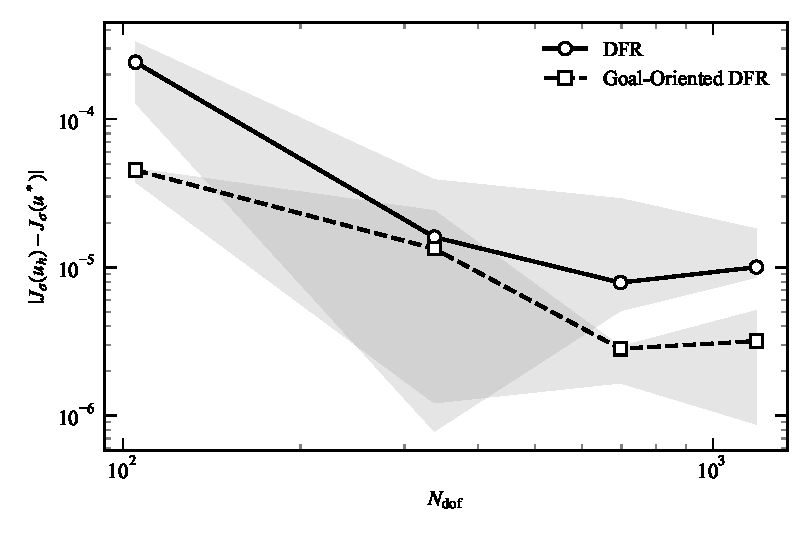
\includegraphics[height=0.70\textheight]{dfr-vs-go-2d}
      \end{center}
    \end{column}
    \begin{column}{0.42\textwidth}
      \vspace{1.5em}
      2D Poisson, point QoI, sweeping the network size:
      \begin{itemize}\itemsep0.6em
        \item Goal-orientation wins \important{33 of 40} runs.
        \item Median QoI error \important{2.3 to 3.9} times smaller (geometric
              mean $3.1\times$).
        \item But this is matched \emph{budget}. Keep it as an upper bound.
      \end{itemize}
    \end{column}
  \end{columns}
\end{frame}

% -----------------------------------------------------------------------------
\begin{frame}{Matched cost: the advantage roughly halves, and splits}
  \begin{columns}[T]
    \begin{column}{0.5\textwidth}
      \important{Two-dimensional sweep: survives.}
      \begin{itemize}\itemsep0.4em
        \item Paired median \good{$2.2\times$}, $95\%$ CI $[1.2, 4.6]$.
        \item Wins \good{28 of 40} runs. Clear of unity.
      \end{itemize}
      \medskip
      \important{Steepness sweep: does not survive.}
      \begin{itemize}\itemsep0.4em
        \item Paired median \alert{$0.92\times$}, CI $[0.69, 1.85]$.
        \item Wins \alert{38 of 80}. Indistinguishable from parity.
      \end{itemize}
    \end{column}
    \begin{column}{0.48\textwidth}
      \centering
      \small
      \begin{tabular}{lcc}
        \toprule
                        & matched      & matched \\
                        & budget       & cost    \\
        \midrule
        2D (size sweep) & $3.1\times$  & $\mathbf{2.2\times}$ \\
        steepness       & up to $15\times$ & $\mathbf{\sim\!1\times}$ \\
        \bottomrule
      \end{tabular}
      \medskip\par
      \footnotesize
      \important{Geometric mean of the QoI-error improvement.} At equal cost the
      steepness advantage vanishes into the seed noise.
    \end{column}
  \end{columns}
  \takeaway{The honest headline: a modest, setting-dependent $\sim\!2\times$ gain
  at equal compute, not an order of magnitude.}
\end{frame}

% -----------------------------------------------------------------------------
\begin{frame}{Why the steepness advantage collapses}
  \begin{columns}[T]
    \begin{column}{0.55\textwidth}
      \begin{center}
        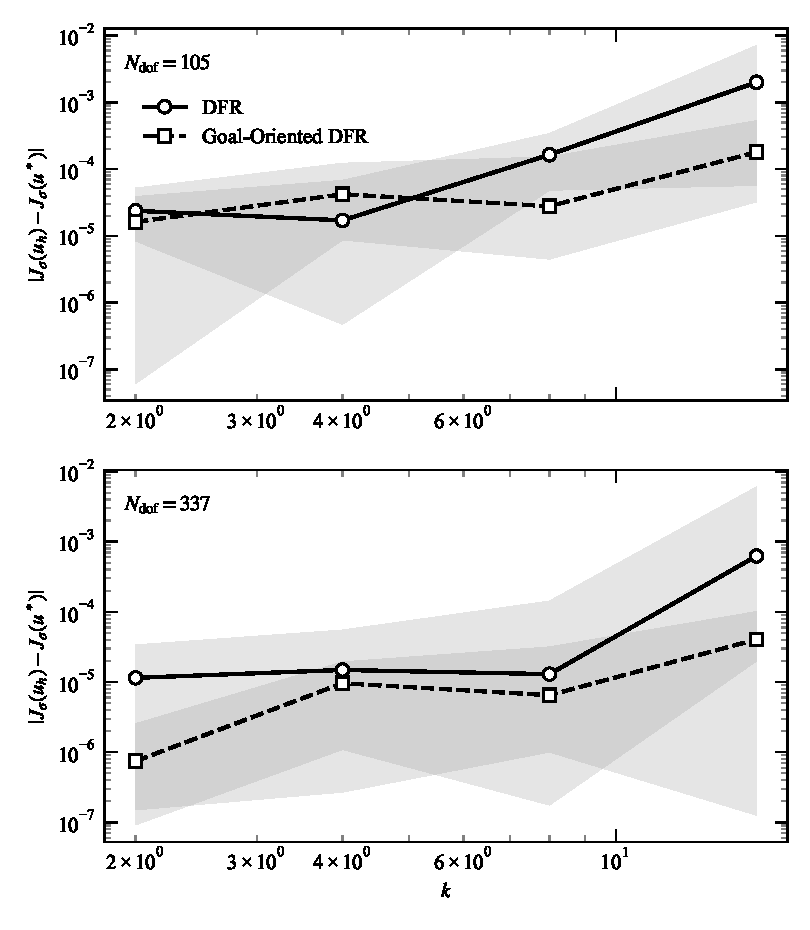
\includegraphics[height=0.72\textheight]{dfr-vs-go-steepness}
      \end{center}
    \end{column}
    \begin{column}{0.43\textwidth}
      \vspace{1.0em}
      \begin{itemize}\itemsep0.7em
        \item At matched budget, plain DFR degrades sharply as the solution
              sharpens; goal-orientation less so.
        \item We had read this as ``the network cannot represent the sharp
              solution.''
        \item At matched cost it is mostly \important{under-convergence}: give
              plain DFR the extra budget and it catches up.
      \end{itemize}
    \end{column}
  \end{columns}
\end{frame}

% =============================================================================
\section{Limits and takeaways}
% =============================================================================

\begin{frame}{What we are not claiming}
  \begin{itemize}\itemsep0.6em
    \item[\alert{$\bullet$}] Plain DFR is \important{not trained to convergence}
          even at $2.5\times$ the budget; a fully converged comparison is out of
          reach at practical budgets.
    \item[\alert{$\bullet$}] The method \important{can hurt}: on easy problems at
          small networks it is worse than the baseline.
    \item[\alert{$\bullet$}] Goal-oriented solutions are $\sim\!10\times$ worse
          \important{globally}. Use them only where the QoI is all you need.
    \item[\alert{$\bullet$}] A single problem family (arctan bumps), a mollified
          point QoI, box domains. Other settings untested.
    \item[\alert{$\bullet$}] The theory predicts \important{none} of the observed
          gain. Explaining it is the open problem this work leaves.
  \end{itemize}
\end{frame}

% -----------------------------------------------------------------------------
\begin{frame}{The bottom line}
  \begin{block}{A carefully delimited contribution}
    \begin{itemize}\itemsep0.4em
      \item A \good{method}: goal-oriented DFR, primal plus adjoint, with the
            stop-gradient that makes it work.
      \item A \good{theorem}: a computable, one-sided reliability bound on the
            QoI error, verified on 168 runs.
      \item A \good{finding}: the loss reallocates accuracy toward the QoI, and
            at equal compute this buys a modest $\sim\!2\times$ in one setting and
            nothing reliable in another.
    \end{itemize}
  \end{block}
  \medskip
  \centering
  \important{A real mechanism, an honest size, and a clear map of where it helps
  and where it does not.}
\end{frame}

% -----------------------------------------------------------------------------
\begin{frame}{Reproduce it}
  Everything is in the repository, one command per figure:
  \medskip
  \begin{itemize}\itemsep0.5em
    \item \code{uv run hp-dfr data all} then \code{uv run hp-dfr figures} for the
          matched-budget sweeps and the bound verification.
    \item \code{uv run hp-dfr data matched-cost} for the equal-cost comparison
          (shardable; runs on the ECS infrastructure in \code{packages/infra}).
    \item Manuscript, code and docs:
          \href{https://github.com/caverac/hp-dfr}{github.com/caverac/hp-dfr},
          \href{https://caverac.github.io/hp-dfr/}{caverac.github.io/hp-dfr}.
  \end{itemize}
  \vfill
  \centering
  \important{Thank you.}
\end{frame}

\end{document}
